As discussed in the previous chapter, we start our investigation by describing a partitioning of loops inspired by software metrics. We state the program's \emph{control flow graph} (CFG) as our program model and give a graph-theoretic definition of \emph{natural loops}, the kind of loops our analysis will handle. Further, we introduce \emph{program slicing}, a standard technique that allows us to extract parts of the CFG that influence termination. Finally, we describe a purely structural metric that counts the number of exits from a loop and introduce three metrics on sliced CFGs.

\section{Control Flow Graphs}

A CFG is a digraph $C = (B, E)$ constructed from the program's source code. CFGs are standard data structures in compiler construction and static analysis, and their construction is discussed in detail in textbooks \cite{DBLP:books/aw/AhoSU86}: The nodes $B$ are so-called \emph{basic blocks} that describe maximal sequences of consecutive statements such that control only enters the basic block through its first statement, and control leaves the block only at its last statement. The flow graph's directed edges $E$ describe the flow of control, i.e.\@ $(a, b) \in E$ if and only if flow of control may enter $b$ from $a$. Each edge $(a, b)$ is labeled with the predicate $assume(a, b)$ guarding its execution, or \true{} if $a$ has a singleton successor. In addition to the basic blocks constructed directly from the program's source code, $B$ contains two nodes \entry{} and \exit{}: The singleton successor to \entry{} is the first executable node of the flow graph. The predecessors to \exit{} are any nodes whose last statement terminates the program. We define two functions on basic blocks $b \in B$: $succs(b)$ returns the set of all immediate successor blocks of $b$ and $preds(b)$ the set of all immediate predecessors of $b$. \Cref{fig:example_program_cfg} shows an example program and its CFG. As in the C programming language edge labels directly correspond to a condition expression in the preceding block, we will sometimes omit edge labels and draw solid edges for labels expressing unnegated conditions, and dashed edges for labels expressing negated conditions.

\sloopy{}, the tool in which we implement our analysis and use in \Cref{ch:experimental} to obtain experimental data, is built on top of \textsc{Clang}, a C language frontend for the \textsc{LLVM} compiler infrastructure. The \textsc{Clang} API allows us to parse a C program and obtain the CFG for each function defined in the program. As prescribed by C semantics, \entry's successor is the singleton entry point of the function and any block after which control leaves the function is a predecessor to \exit{}. Due to this handling of CFGs in \textsc{Clang}, our analysis is intra-procedural.

\begin{figure}
\begin{subfigure}{.58\linewidth}
    \cfile{figures/test.c}
\end{subfigure}
\hfill
\begin{subfigure}{.38\linewidth}
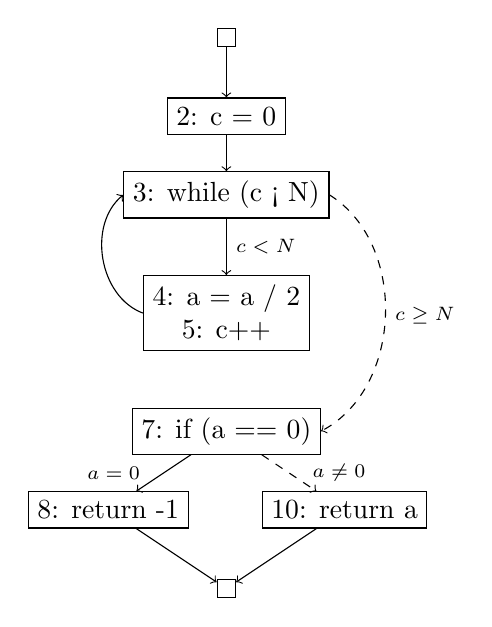
\begin{tikzpicture}[%
    ->,
    box/.style={draw, rectangle, align=center}
  ]
\node[box] (entry) at (0,0) {\entry};
\node[box] (2) at (0,-1) {2: c = 0};
\node[box] (3) at (0,-2) {3: while (c < N)};
\node[box] (4) at (0,-3.5) {4: a = a / 2\\5: c++};
\node[box] (7) at (0,-5) {7: if (a == 0)};
\node[box] (8) at (-1.5,-6) {8: return -1};
\node[box] (10) at (1.5,-6) {10: return a};
\node[box] (exit) at (0,-7) {\exit};
\path[->,every node/.style={font=\scriptsize}]
      (entry) edge (2)
      (2) edge (3)
      (3) edge[right] node {$c < N$} (4)
      (3.east) edge[dashed, bend left=60, right] node {$c \ge N$} (7.east)
      (4.west) edge[bend left=60] (3.west)
      (7) edge[left] node[xshift=-0.5em] {$a = 0$} (8)
      (7) edge[dashed, right] node[xshift=0.5em] {$a \ne 0$} (10)
      (8) edge (exit)
      (10) edge (exit);
\end{tikzpicture}
\end{subfigure}
    \caption{Example program and its CFG.}
    \label{fig:example_program_cfg}
\end{figure}

\section{Natural Loops}

Having defined the CFG as the underlying data structure for analysis, we now describe loops in terms of graph-theoretic notions. While a straight-forward definition might consider any cycle in the CFG a loop, this is too lax for the purposes of static analysis. Intuitively, a loop should have a single entry point, and its edges should form at least one cycle. The graph-theoretic definition of these properties is the \emph{natural loop}. We first define the \emph{dominator relation} and \emph{back edges}, which we then use to define the natural loop. Our definitions follow those presented in \cite{DBLP:books/aw/AhoSU86}.

\begin{definition}[Dominator relation]
    A node $d$ of a flow graph \emph{dominates} a node $n$ ($d \text{ dom }n$) if and only if every path from \entry{} to $n$ goes through $d$.
\end{definition}

\begin{definition}[Back edge]
    A \emph{back edge} is an edge $a \rightarrow b$ whose head $b$ dominates its tail $a$.
\end{definition}

\begin{definition}[Natural loop]
Given a back edge $n \rightarrow d$, its \emph{pre loop} consists of $d$ plus the set of nodes that can reach $n$ without going through $d$. We call $d$ the \emph{header} of the loop. The \emph{natural loop} $L$ with header $d$ is the union of all pre loops with header $d$ (see \Cref{fig:same_header} for a simple example). A path $p$ through $L$ is any path $d, b_1, b_2, \dots, b_n, d$ where $b_i \in L$ and $b_i \ne d$ for $1 \le i \le n$. For the set of all such paths, we write $p \in paths(L)$.
\end{definition}

\begin{figure}
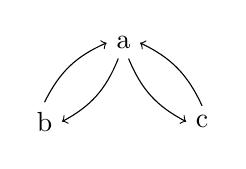
\begin{tikzpicture}[->]
\node (a) at (0,0) {a};
\node (b) at (-1,-1) {b};
\node (c) at (1,-1) {c};
\path (a) edge[bend left=20] (b.east)
      (a) edge[bend right=20] (c.west)
      (b.north) edge[bend left=20] (a.west)
      (c.north) edge[bend right=20] (a.east);
\end{tikzpicture}
\caption{A natural loop with header $a$ consisting of two pre loops with the back edges $b \rightarrow a$ and $c \rightarrow a$.}
\label{fig:same_header}
\end{figure}

\begin{definition}[Nested loop]
Two natural loops are either disjoint or one is entirely contained within the other. In the latter case, we call the contained loop a \emph{nested} or \emph{inner loop}.
\end{definition}

As our analysis is CFG-based, it remains to define the control flow graph of a natural loop:

\begin{definition}[Control flow graph of a natural loop]
A natural loop $L$'s control flow graph $C_L$ is exactly the control flow graph of the subprogram defining the natural loop. To construct $C_L$, we start from the subgraph of the function's CFG $C_F$ whose vertex set equals $L$. To this subgraph we add fresh \entry{} and \exit{} nodes, introduce an edge $(\entry, d)$ where $d$ is the header of $L$, and introduce an edge $(a, \exit)$ for each edge $(a, b), a \in L, b \not\in L$ in $C_F$ with the same edge label $assume(a, b)$.
\label{def:nlcfg}
\end{definition}

\begin{figure}
\begin{subfigure}{.58\linewidth}
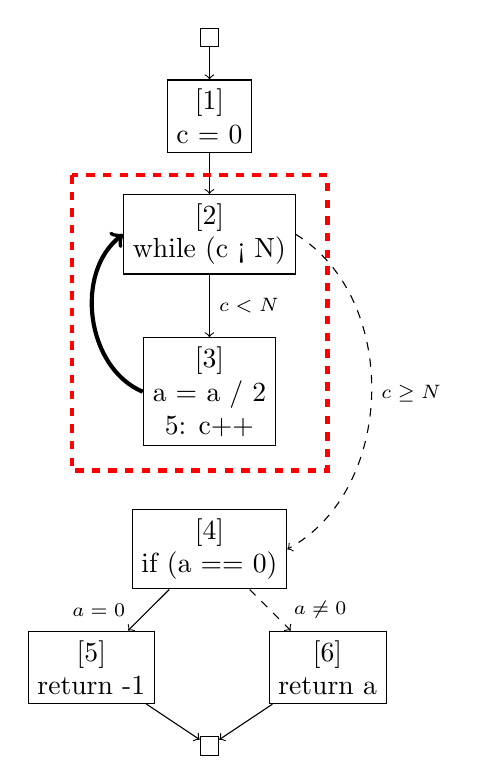
\begin{tikzpicture}[%
    ->,
    box/.style={draw, rectangle, align=center}
  ]
\node[box] (entry) at (0,0) {\entry};
\node[box] (2) at (0,-1) {[1]\\c = 0};
\node[box] (3) at (0,-2.5) {[2]\\while (c < N)};
\node[box] (4) at (0,-4.5) {[3]\\a = a / 2\\5: c++};
\node[box] (7) at (0,-6.5) {[4]\\if (a == 0)};
\node[box] (8) at (-1.5,-8) {[5]\\return -1};
\node[box] (10) at (1.5,-8) {[6]\\return a};
\node[box] (exit) at (0,-9) {\exit};
\draw[rectangle,dashed,red,line width=1.5pt] (-1.75,-1.75) rectangle (1.5,-5.5);
\path[->,every node/.style={font=\scriptsize}]
      (entry) edge (2)
      (2) edge (3)
      (3) edge[right] node {$c < N$} (4)
      (3.east) edge[dashed, bend left=60, right] node {$c \ge N$} (7.east)
      (4.west) edge[bend left=60,line width=1.5pt] (3.west)
      (7) edge[left] node[xshift=-0.5em] {$a = 0$} (8)
      (7) edge[dashed, right] node[xshift=0.5em] {$a \ne 0$} (10)
      (8) edge (exit)
      (10) edge (exit);
\end{tikzpicture}
    \caption{CFG of function \texttt{test} in \Cref{fig:example_program_cfg}. The backedge $[3] \rightarrow [2]$ and its natural loop are highlighted.}
    \label{fig:example_loop_cfga}
\end{subfigure}
\hfill%
\begin{subfigure}{.38\linewidth}
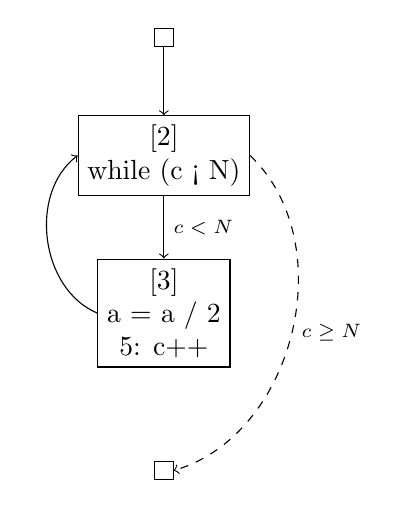
\begin{tikzpicture}[%
    ->,
    box/.style={draw, rectangle, align=center}
  ]
\node[box] (entry) at (0,-1) {\entry};
\node[box] (3) at (0,-2.5) {[2]\\while (c < N)};
\node[box] (4) at (0,-4.5) {[3]\\a = a / 2\\5: c++};
\node[box] (exit) at (0,-6.5) {\exit};
\path[->,every node/.style={font=\scriptsize}]
      (entry) edge (3)
      (3) edge[right] node {$c < N$} (4)
      (3.east) edge[dashed, bend left=60, right] node {$c \ge N$} (exit.east)
      (4.west) edge[bend left=60] (3.west);
\end{tikzpicture}
    \caption{CFG of the natural loop of backedge $[3] \rightarrow [2]$.}
    \label{fig:example_loop_cfgb}
\end{subfigure}
\caption{Control flow graph of a natural loop.}
\end{figure}

\begin{example}
\Cref{fig:example_loop_cfga} shows the CFG of function \texttt{test} from \Cref{fig:example_program_cfg} and highlights the singleton backedge as well as its natural loop. \Cref{fig:example_loop_cfgb} shows the natural loop's CFG constructed according to \Cref{def:nlcfg}.
\end{example}

\subsection{Irreducible Flow Graphs}
In \emph{reducible flow graphs}, all cycles are natural loops, i.e.\ each cycle has a single entry point (the natural loop's header) that dominates all basic blocks in the cycle. \emph{Irreducible flow graphs} contain one or more loops with multiple entry points. By restricting our analysis to natural loops, we ignore loops with such irreducible flow graphs. We argue that this restriction is tolerable for two reasons:

\begin{enumerate}
    \item A recent study by \citeauthor{DBLP:journals/spe/StanierW12} \cite{DBLP:journals/spe/StanierW12} "found 5 irreducible functions in a total of \num{10427}, giving a total average irreducibility for this set of current programs of 0.048\%". The authors conclude that irreducibility "is an extremely rare occurrence, and it will probably be even rarer in the future".
    \item Many static analysis tools are restricted to reducible CFGs. In particular, our main tool for comparison, \loopus, only supports reducible CFGs at the moment.
\end{enumerate}

\section{Program Slicing}
\label{sec:slicing}

Classic software metrics can be divided into \emph{size counts} (e.g.\ lines of code, LOC) and \emph{software complexity measures} (e.g.\ cyclometic complexity, measuring the number of linearly independent paths) \cite{DBLP:journals/jss/FentonN99}. However, we cannot directly compute such measures and hope to find correlation with the difficulty to prove termination: A long program may perform many auxiliary computations not influencing termination -- on the other hand, a short program may perform a few intricate operations that make an automated termination proof difficult. Thus, an overly simple approach that computes measures on the original program cannot yield a proper classification.

\begin{figure}
\begin{subfigure}[t]{.52\linewidth}
\begin{tikzpicture}[%
    ->,
    node distance=0.5,
    box/.style={draw, rectangle, align=center}
  ]
\node[box] (0) at (0,0) {\entry};
\node[box, below=of 0] (1) {[1]\\c = 0\\r = 0};
\node[box, below=of 1] (2) {[2]\\while (c < N)};
\node[box, below=of 2] (3) {[3]\\if (c \% 2)};
\node[box, below left=of 3,xshift=0.5cm] (4) {[4]\\r += c};
\node[box, below right=of 3,xshift=-0.5cm] (5) {[5]\\r += 2};
\node[box, below=of 3,yshift=-1cm] (6) {[6]\\c++};
\node[box, below=of 6] (exit) {\exit};
\path (0) edge (1)
      (1) edge (2)
      ($(2.south)+(-0.25,0)$) edge[blue] ($(3.north)+(-.25,0)$)
      ($(2.south)+(0.25,0)$) edge[red] ($(3.north)+(.25,0)$)
      (3) edge[blue] (4)
      (3) edge[dashed,red] (5)
      (4) edge[blue] (6)
      (5) edge[red] (6)
      (6) edge[out=180, in=180, looseness=2] (2)
      (2) edge[dashed, out=0, in=0, looseness=1] (exit);
\end{tikzpicture}
\caption{A program with two paths $p_1, p_2$ that don't influence its termination. $p_1$ is shown in blue, $p_2$ in red.}
\label{fig:requires_slicing_a}
\end{subfigure}
\hfill
\begin{subfigure}[t]{.44\linewidth}
\begin{tikzpicture}[%
    ->,
    node distance=0.5,
    box/.style={draw, rectangle, align=center}
  ]
\node[box] (0) at (0,0) {\entry};
\node[box, below=of 0] (1) {[1]\\c = 0\\};
\node[box, below=of 1] (2) {[2]\\while (c < N)};
\node[box, below=of 3,yshift=-1cm] (6) {[6]\\c++};
\node[box, below=of 6] (exit) {\exit};
\path (0) edge (1)
      (1) edge (2)
      (2) edge (6)
      (6) edge[out=180, in=180] (2)
      (2) edge[dashed, out=0, in=0] (exit);
\end{tikzpicture}
\caption{The sliced program containing only variables and statements relevant to termination.}
\label{fig:requires_slicing_b}
\end{subfigure}
\caption{Program slicing.}
\label{fig:requires_slicing}
\end{figure}


\begin{example}
Consider the flow graph in \Cref{fig:requires_slicing_a}: While there are two paths, $p_1 = (2 \rightarrow 3 \rightarrow 4 \rightarrow 6)$ and $p_2 = (2 \rightarrow 3 \rightarrow 5 \rightarrow 6)$, for the loop's termination it is irrelevant which path is taken. More precisely, the loop's termination depends on the expression in block [2], and as such on the variables \texttt{c} and \texttt{N}. As neither \texttt{c} nor \texttt{N} are written in blocks [4] and [5], whether path $p_1$ or $p_2$ is executed, is irrelevant to the loop's termination. \Cref{fig:requires_slicing_b} shows a program slice ignoring statements not relevant to termination.
\end{example}

\emph{Program slicing} is a method first described by \citeauthor{DBLP:conf/icse/Weiser81} \cite{DBLP:conf/icse/Weiser81}:

\begin{definition}[Program state, program trace]
    Let $P$ be a program and $V$ the set of variable names occurring in $P$. A \emph{program state} of $P$ is a tuple $(n, q)$ where $n$ is a program location in $P$ and $q$ is a function mapping variable names to their values. A \emph{program trace} is a sequence $(n_0, q_0), (n_1, q_1), \dots$ of program states.
\end{definition}
\begin{definition}[Slicing criterion, program slice]
    A \emph{slicing criterion} $C = \langle l, V \rangle$, where $l$ is a program location and $V$ is a set of variables to observe at $l$, defines a projection of program states \[
        \text{Proj}_{\langle l, V \rangle}(n, q) = \begin{cases}
            \varepsilon & \text{if } n \ne l \\
            (n, q|V) & \text{otherwise}
        \end{cases}
    \]
where $\varepsilon$ is the empty string and $q|V$ is $q$ restricted to domain $V$. We extend the projection to traces:
\[
    \text{Proj}_{\langle l, V \rangle}(s_0, s_1, \dots) = \text{Proj}_{\langle l, V \rangle}(s_0), \text{Proj}_{\langle l, V \rangle}(s_1), \dots
\]

Given a program $P$ and an input $I$, let $T(P, I)$ denote the trace of running $P$ on $I$. A \emph{program slice} $P'$ with respect to slicing criterion $C$ is any program obtained by removing statements from $P$, such that $\text{Proj}_C(T(P, I)) = \text{Proj}_C(T(P', I))$.
\end{definition}

\citeauthor{DBLP:conf/icse/Weiser81} \cite{DBLP:conf/icse/Weiser81} also defines a fixed point iteration algorithm to compute program slices.

\subsection{Termination Slicing Criteria}

Because a loop may be exited at multiple locations, a slicing criterion specifying a window for observing loop termination has to consider multiple program locations. Thus, we adapt Weiser's definition of a slicing criterion to a \emph{generalized slicing criterion} $C' = \{ (l, V) \mid l \text{ is a program location, and } V \text{ is a set of variables} \}$, i.e.\ $C'$ is a set of slicing criteria. A generalized slicing criterion observing loop termination for a natural loop's flow graph is given by
\[
    C_{term} = \bigcup \limits_{P\,\in\,preds(\exit)} \big\{ (P, \{ v \mid v \text{ is a variable in } assume(P, \exit) \}) \big\}
\]

Intuitively, the criterion observes the value of any variable in the conditions guarding termination. From now on, when referring to a sliced program, we mean a program sliced with respect to criterion $C_{term}$. Weiser's original algorithm can easily be adapted to deal with a generalized slicing criterion. We give a non-trivial example for slicing with respect to $C_{term}$:

\begin{example}
    \Cref{fig:slicing_ex_a} shows a loop statement adapted from \texttt{rpe.c} in the cBench benchmark suite \cite{cBench}, and \Cref{fig:slicing_ex_b} the CFG of the corresponding natural loop. Program locations defined in the slicing criterion, i.e.\ the predecessors to \exit{} -- blocks [2] and [6] -- are included in the slice by default, as they directly control termination. We apply a red frame to statements included in the slice.

We then compute the preliminary set of relevant variables for each statement -- clearly, from the definition of a slicing criterion, for each pair $(l, V) \in C_{term}$, all $v \in V$ are relevant at $l$. For $C_{term}$ this means \texttt{i}, obtained from the edge label $assume(2,\exit): i > 5$, is relevant at block [2], \texttt{exp} referenced in $assume(6,\exit): exp > 5$ is relevant at block [6]. For any other statement $n$, we have to consider its immediate successors: If variable $v$ is relevant at an immediate successor $m$ and $v$ is defined at $n$, then all variables referenced in defining $v$ are relevant at $n$. For an example, see block [8]: \texttt{exp} is relevant in [9] and defined in [8], thus \texttt{exp} is no longer relevant, but \texttt{d}, which is referenced to define \texttt{exp}, is. If $v$ is relevant at successor $m$ but not defined at $n$, $v$ is still relevant at $n$. For an example, refer to block [7]: no variables are defined, thus it inherits its relevant variables from both [8] and [9]. \Cref{fig:slicing_ex_c} shows the relevant variables after this step -- for simplicity we summarize the relevant variables for all statements of a block in parentheses.

Next, we compute the preliminary set of statements to include in the slice: These are all statements $n$ defining a variable $v$ that relevant in an immediately succeeding statement. There are two statements of this kind: the assignment of \texttt{exp} in block [8] and the increment of \texttt{i} in block [9]. Thus, we include them in the slice, in addition to the statements from blocks [2] and [6] that were included from the beginning. \Cref{fig:slicing_ex_c} highlights all statements included in the slice after this step with a red frame.


So far, we have only considered statements directly influencing the slicing criterion. Consider block [7], which decides if the statement in block [8], which we already included in the slice, is executed -- we say [8] is \emph{control-dependent} on [7]. Thus, we add those branch statements to the slice that statements already included in the slice are control-dependent on, and introduce a \emph{branch statement criterion} $(b, REF(b))$ for each such branch statement $b$ where $REF(b)$ is the set of variables referenced in $b$. To illustrate why this is necessary, consider block [7]: variable \texttt{itest} controls subsequent execution of statements in the slice, thus we need to observe its value at this location.

We re-iterate computation of relevant variables and statements included in the slice with respect to the already computed relevant variables, and all variables relevant to newly introduced branch slicing criteria until a fixed point is reached. \Cref{fig:slicing_ex_d} shows the statements ultimately included in the slice: Lines 5--9 of the original program are not included, because \texttt{mant}, and thus the \texttt{if} statement on line 5 have no influence on the loop's termination.
\end{example}

\begin{figure}
    \begin{subfigure}{.48\linewidth}
        % cBench_preprocessed_release29_2013_09_18_Merged/telecom_gsm/src/rpe.c -func APCM_quantization -lines 485,
        \begin{ccode*}{fontsize=\small}
for (i = 0; i <= 5; i++) {
    itest |= temp <= 0;
    temp = temp >> 1;

    if (temp) {
        mant++;
    } else {
        mant--;
    }

    if (exp > 5)
        return;

    if (itest == 0)
        exp = d;
}
\end{ccode*}
        \caption{A loop statement adapted from \texttt{rpe.c} in the cBench benchmark.}
        \label{fig:slicing_ex_a}
    \end{subfigure}
    \hfill
    \begin{subfigure}{.48\linewidth}
        \begin{tikzpicture}[%
            font=\small,
            ->,
            node distance=0.4,
            every node/.style={draw, rectangle, align=center}
            ]
            \node (0) at (0,0) {\entry};
            \node[below=of 0] (2) {[2]\\for (...; \fcolorbox{red}{white}{i <= 5}; ...)};
            \node[below=of 2] (3) {[3]\\itest |= temp <= 0;\\temp = temp >{}> 1\\if (temp)};
            \node[below=of 3] (4) {[4]\\mant++;};
            \node[below right=of 3,xshift=-0.5cm] (5) {[5]\\mant-{}-;};
            \node[below=of 5] (6) {[6]\\\fcolorbox{red}{white}{if (exp > 5)}};
            \node[left=of 6] (7) {[7]\\if (itest == 0)};
            \node[below left=of 3] (8) {[8]\\exp = d;};
            \node[above=of 8,yshift=0.8cm] (9) {[9]\\i++;};
            \node[above right=of 2] (exit) {\exit};
            \path (0) edge (2)
            (2) edge (3)
            (3) edge (4)
            (3) edge[dashed] (5)
            (4) edge (6)
            (5) edge (6)
            (6) edge[dashed] (7)
            (7) edge[out=180,in=270] (8)
            (7) edge[dashed] (9)
            (8) edge (9)
            (9) edge[out=90,in=180] (2)
            (2) edge[dashed,in=180] (exit);
            \draw ($(6.north)+(0.8,0)$) .. controls +(up:4cm) and +(right:1cm) .. (exit);
        \end{tikzpicture}
        \caption{The corresponding natural loop's CFG.}
        \label{fig:slicing_ex_b}
    \end{subfigure}
    \begin{subfigure}{.48\linewidth}
        \begin{tikzpicture}[%
            font=\small,
            ->,
            node distance=0.4,
            every node/.style={draw, rectangle, align=center}
            ]
            \node (0) at (0,0) {\entry};
            \node[below=of 0] (2) {[2] (i, exp, d)\\for (...; \fcolorbox{red}{white}{i <= 5}; ...)};
            \node[below=of 2] (3) {[3] (i, exp, d)\\itest |= temp <= 0;\\temp = temp >{}> 1\\if (temp)};
            \node[below=of 3] (4) {[4] (i, exp, d)\\mant++;};
            \node[below right=of 3,xshift=-0.5cm] (5) {[5] (i, exp, d)\\mant-{}-;};
            \node[below=of 5] (6) {[6] (i, exp, d)\\\fcolorbox{red}{white}{if (exp > 5)}};
            \node[left=of 6] (7) {[7] (i, exp, d)\\if (itest == 0)};
            \node[below left=of 3,xshift=-0.2cm] (8) {[8] (i, d)\\\fcolorbox{red}{white}{exp = d;}};
            \node[above=of 8,yshift=0.8cm] (9) {[9] (i, exp)\\\fcolorbox{red}{white}{i++;}};
            \node[above right=of 2] (exit) {\exit{}};
            \path (0) edge (2)
            (2) edge (3)
            (3) edge (4)
            (3) edge[dashed] (5)
            (4) edge (6)
            (5) edge (6)
            (6) edge[dashed] (7)
            (7) edge[out=180,in=270] (8)
            ($(7.north)-(1,0)$) edge[dashed] (9)
            (8) edge (9)
            (9) edge[out=90,in=180] (2)
            (2) edge[dashed,in=180] (exit);
            \draw (6.east) .. controls +(right:0.2cm) and +(right:1.5cm) .. (exit);
        \end{tikzpicture}
        \caption{The CFG after one iteration of Weiser's algorithm.}
        \label{fig:slicing_ex_c}
    \end{subfigure}
    \hfill%
    \begin{subfigure}{.48\linewidth}
        \begin{tikzpicture}[%
            font=\small,
            ->,
            node distance=0.4,
            every node/.style={draw, rectangle, align=center}
            ]
            \node (0) at (0,0) {\entry};
            \node[below=of 0] (2) {[2]\\for (...; \fcolorbox{red}{white}{i <= 5}; ...)};
            \node[below=of 2] (3) {[3]\\\fcolorbox{red}{white}{itest |= temp <= 0;}\\\fcolorbox{red}{white}{temp = temp >{}> 1;}\\if (temp)};
            \node[below=of 3] (4) {[4]\\mant++;};
            \node[below right=of 3,xshift=-0.5cm] (5) {[5]\\mant-{}-;};
            \node[below=of 5] (6) {[6]\\\fcolorbox{red}{white}{if (exp > 5)}};
            \node[left=of 6] (7) {[7]\\\fcolorbox{red}{white}{if (itest == 0)}};
            \node[below left=of 3,xshift=-0.2cm] (8) {[8]\\\fcolorbox{red}{white}{exp = d;}};
            \node[above=of 8,yshift=0.8cm] (9) {[9]\\\fcolorbox{red}{white}{i++;}};
            \node[above right=of 2] (exit) {\exit};
            \path (0) edge (2)
            (2) edge (3)
            (3) edge (4)
            (3) edge[dashed] (5)
            (4) edge (6)
            (5) edge (6)
            (6) edge[dashed] (7)
            (7) edge[out=180,in=270] (8)
            (7) edge[dashed] (9)
            (8) edge (9)
            (9) edge[out=90,in=180] (2)
            (2) edge[dashed,in=180] (exit);
            \draw ($(6.north)+(0.9,0)$) .. controls +(up:4cm) and +(right:1cm) .. (exit);
        \end{tikzpicture}
        \caption{The fixed point computed by Weiser's algorithm.}
        \label{fig:slicing_ex_d}
    \end{subfigure}
    \caption{An example for the termination slicing process.}
    \label{fig:slicing_ex}
\end{figure}

\section{Metric-based Classification}
\label{sec:class_cfg}

Basic structural classification inspired by classic software metrics can be defined on the CFG. \citeauthor{DBLP:conf/sas/ZulegerGSV11} \cite{DBLP:conf/sas/ZulegerGSV11} consider loops with exactly one path (in the program slice) as \emph{trivial}. While determining the class of loops with a single path is linear in the number of basic blocks, for more than one path this notion becomes undesirable for our purposes for two reasons:
\begin{enumerate}
    \item If we consider all paths, the number of paths may still be countably infinite, caused by the presence of a nested loop.
    \item If we restrict our definition to all simple paths, counting them is hard (shown \emph{\#P-complete} in \cite{DBLP:journals/siamcomp/Valiant79} for general graphs -- we do not know of a result for reducible graphs).
\end{enumerate}

Rather than counting the paths of a loop, we will therefore consider the number of exits from the loop, in terms of software metrics a size count:

\begin{definition}
    Let $\mathcal{L}$ denote the set of all loops. Then $\mathcal{L}^{E=i}$ is defined as the class of loops with $i$ exits, i.e.\@ $\mathcal{L}^{E=i} = \{ L \in \mathcal{L} \,\mid\, |preds(\exit)| = i \}$.
\end{definition}

One may also impose other relations than equality to describe loops with a number of exits from an interval, as demonstrated in \Cref{fig:exit_hierarchy}.

\def\cg{(2.5cm,0) ellipse (6cm and 3cm)}
\def\cc{(1cm,0) ellipse (4cm and 2.5cm)}
\def\cb{(0.5cm,0) ellipse (3cm and 2cm)}
\def\cp{(0,-0.5cm) ellipse (2cm and 1cm)}
% \def\ca{(0,0.5cm) ellipse (2cm and 1cm)}
\def\ca{(0,0) ellipse (2cm and 1cm)}

\begin{figure}[h]
\begin{tikzpicture}
    \begin{scope}
        \fill[cyan] \cg;
        \fill[green] \cc;
        \fill[yellow] \cb;
        % \fill[red,opacity=0.8] \cp;
        \fill[orange,opacity=0.8] \ca;
        \draw \cg;
        \node at (9.5cm,0) {$\dots$};
        \node at (7.75cm,0) {$\mathcal{L}^{E \le n}$};
        \node at (6.5cm,0) {$\dots$};
        \draw \cc;
        \node at (4.25cm,0) {$\mathcal{L}^{E \le 2}$};
        \draw \cb;
        \node at (2.75cm,0) {$\mathcal{L}^{E \le 1}$};
        % \draw \cp;
        % \node at (0,-1cm) {$\mathcal{L}^{P_1}$};
        \draw \ca;
        \node at (0,0) {$\mathcal{L}^{E = 0}$};
    \end{scope}
\end{tikzpicture}

\caption{Loops with at most $i$ exits $\mathcal{L}^{E \le i}$ are totally ordered under inclusion.}
\label{fig:exit_hierarchy}
\end{figure}

\subsection{Slice-based Metrics}
\label{sub:slice_based_class}

Software metrics and their measurement are a long standing topic of discussion in the software engineering community, and many metrics routinely used in industry have been dismissed as inconclusive for various reasons \cite{DBLP:journals/jss/FentonN99}. In his original paper \cite{DBLP:conf/icse/Weiser81}, \citeauthor{DBLP:conf/icse/Weiser81} lists a number of slicing-based metrics. As only computation influencing termination remains in a sliced program, we can consider an additional size count and two complexity metrics of the loop:

\begin{description}
    \item[Number of basic blocks] The number of basic blocks in the sliced CFG. This is merely measuring size of the slice, but because it is adjusted for termination, it is more meaningful than just referring to lines of code (LOC).
    \item[Nesting depth] The depth of a depth-first spanning tree of the sliced CFG. This is a complexity software metric. Intuitively, there should be a reason for the programmer to introduce additional branches influencing termination, and we want to study if there is a correlation to the difficulty of proving termination.
    \item[Control variables] The number of variables affecting what is observed through the slicing criterion $C_{term}$. For this metric, we compute the union of relevant variables over all statements. Another complexity metric, this gives an estimate of how intricate the computation controlling the terminating branch statements is.
\end{description}
